
\clearpage

$\ $
\vspace{14.5cm}

\noindent\begin{tabular}{p{0.9cm}p{6.8cm}}
& 2015.$\,$ Guatemala, Centro América \\
&\Bold Instituto Nacional de Estadística\\[-0.4cm]
&\color{blue!50!black}\url{www.ine.gob.gt}\\[0.9cm]
\end{tabular}\\
\noindent\begin{tabular}{p{0.9cm}p{6.8cm}}
& Está permitida la reproducción parcial o total de los contenidos de este documento con la mención de la fuente. \\[0.5cm]
 
& Este documento fue elaborado empleando  {\Sans R}, Inkscape y {\Logos \XeLaTeX}.\\
\end{tabular} 
\pagestyle{empty}

\clearpage


	%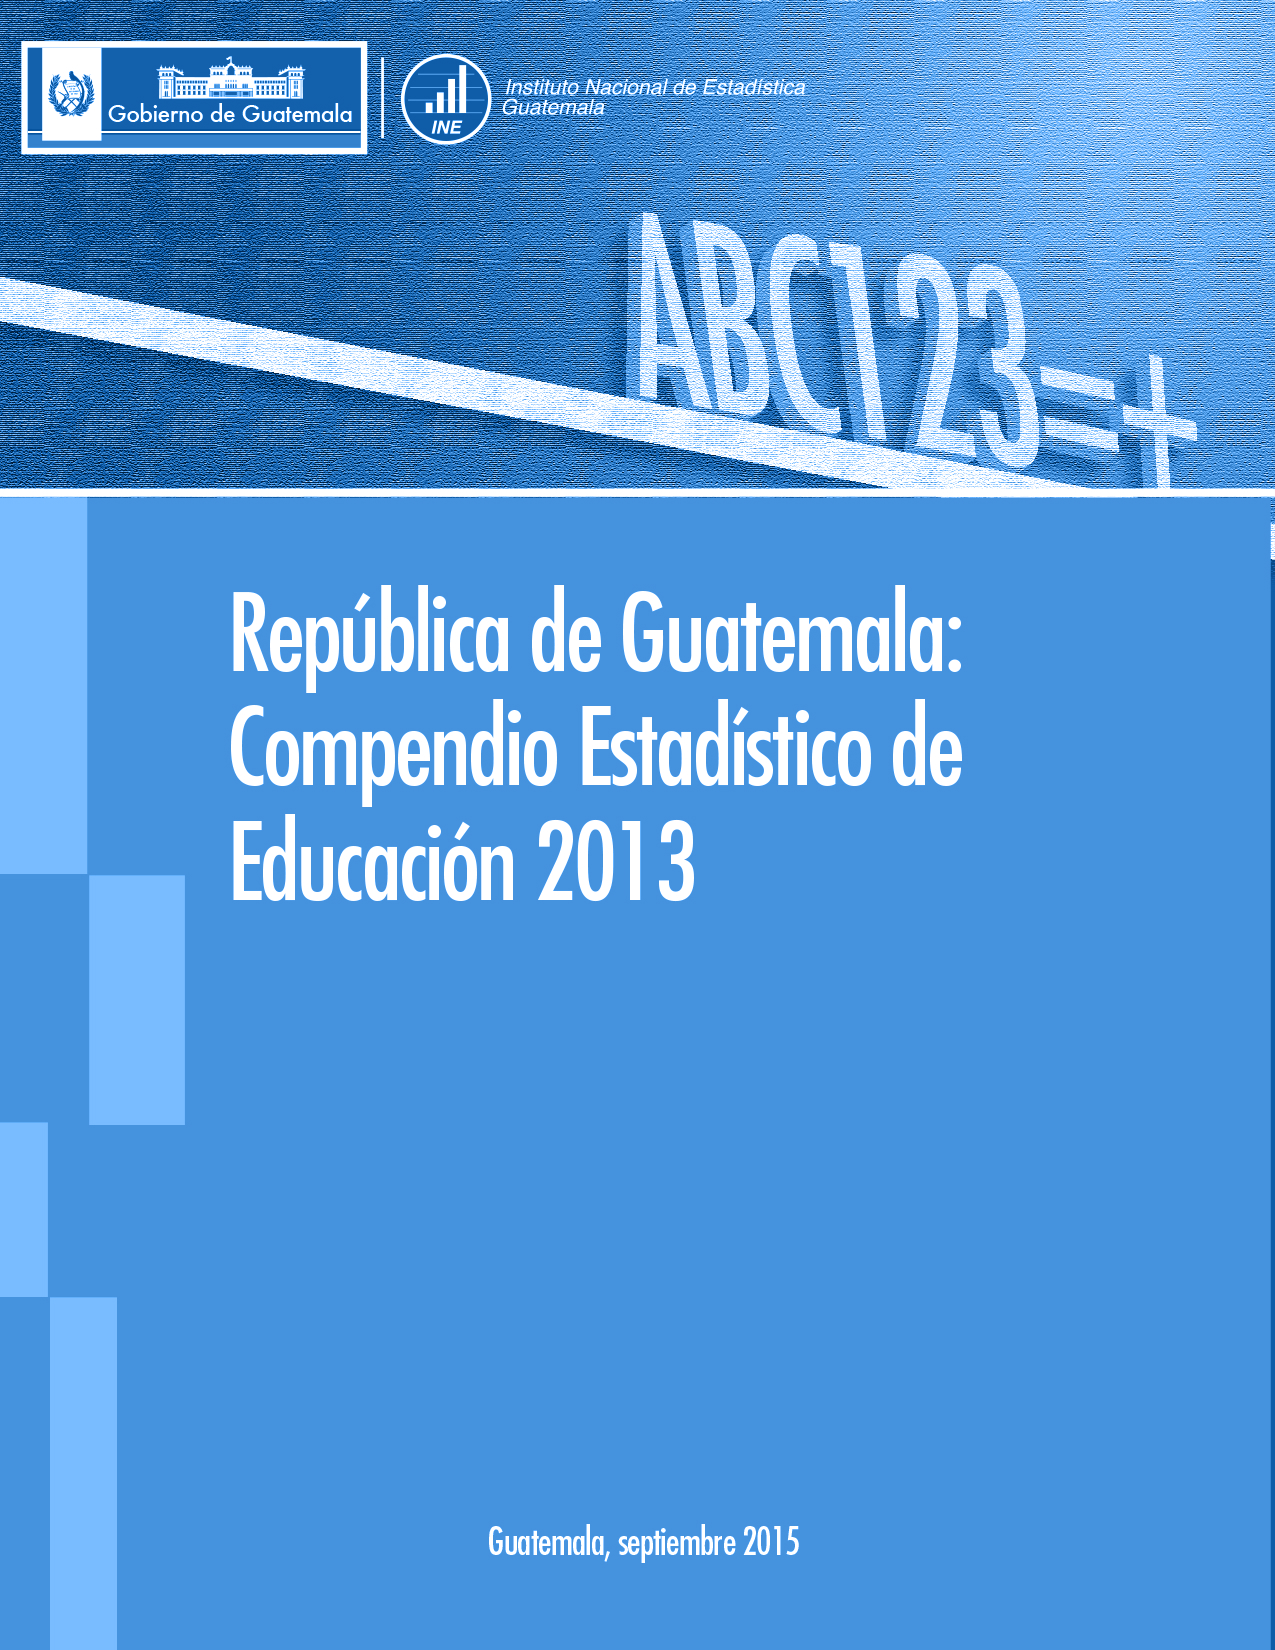
\includepdf{educativa_interior.pdf}
	
	\clearpage
	\newpage $\ $
	\newpage $\ $
$\ $
\vspace{7cm}

\begin{center}
\Bold \LARGE COMPENDIO DE ESTADÍSTICAS DE EDUCACIÓN 2014 \\
\end{center}
\cleardoublepage
$\ $
\vspace{0.0cm}

\begin{center}
	{\Bold \LARGE AUTORIDADES}\\[1cm]
	
	
	{\Bold \large \color{color1!89!black} JUNTA  DIRECTIVA} \\[0.4cm]
	
	{ \Bold Ministerio de Economía}  		\\ 
	Titular: Jorge Méndez Herbruger   \\ 
	Suplente: Jacobo Rey Sigfrido Lee Leiva  \\ [0.4cm] 
	
	{\Bold Ministerio de Finanzas} \\ 
	Titular: Dorval José Carías Samayoa \\ 
	Suplente: Edwin Oswaldo Martínez Cameros\\[0.4cm] 
	
	{\Bold Ministerio de Agricultura, Ganadería y Alimentación} \\ 
	Titular: José Sebastian Marcucci Ruíz   \\ 
	Suplente: Henry Giovanni Vásquez Kilkan \\ [0.4cm] 
	
	{\Bold Ministerio de Energía y Minas}\\ 
	Titular: Juan Pablo Ligorría Arroyo \\ 
	Suplente: Jorge David Calvo Drago\\ [0.4cm]
	{\Bold Secretaría de Planificación y Programación de la Presidencia}   \\
	Titular: Ekaterina Arbolievna Parrilla Artuguina   \\ 
	Suplente: Dora Marina Coc Yup\\ [0.4cm] 
	{\Bold Banco de Guatemala} \\ 
	Titular: Julio Roberto Suárez Guerra \\ 
	Suplente: Sergio Francisco Recinos Rivera\\ [0.4cm] 
	{\Bold Universidad de San Carlos de Guatemala de Guatemala} \\ 
	Titular: Murphy Olimpo Paiz Recinos   \\
	Suplente: Oscar René Paniagua Carrera  \\ [0.4cm]
	{\Bold Universidades Privadas} \\
	Titular: Miguel Ángel Franco de León \\			 Suplente: Ariel Rivera Irías\\ [0.4cm] 
	{\Bold Comité Coordinador de \ Asociaciones  Agrícolas, Comerciales,Industriales y Financieras} \\ 
	Titular: Juan Raúl Aguilar Kaehler \\
	Suplente:  Oscar Augusto Sequeira García  \\ [0.4cm]
	
	{\Bold \large \color{color1!89!black} GERENCIA}\\[0.2cm]
	Gerente:  Rubén Darío Narciso Cruz		\\
	Subgerente Técnico:  Jaime Roberto Mejía Salguero\\
	Subgerente Administrativo Financiero:  Orlando Roberto Monzón Girón\\ 
\end{center}
\cleardoublepage
$\ $
\vspace{-0.3cm}

		\begin{center}
			{\Bold \LARGE Oficina Coordinadora Sectorial de Estadísticas de Educación}\\[.3cm]
			{\Bold \LARGE OCSE - Educación}\\[1cm]
		\end{center}

\begin{multicols}{2}

\begin{center}

	

	\textbf{Instituto Nacional de Estadística}\\
	Coordinador: Gerson Palacios Pantaleón\\ [0.4cm]
	
\textbf{	Secretaría Presidencial de la Mujer – SEPREM}\\
	Titular: Crisalda Lorena Rivera Diaz \\
	Suplente: Mayra López\\ [0.4cm]
	
\textbf{	Secretaría de Planificación y Programación de la Presidencia – SEGEPLAN}\\
	Titular: Edna Abigail Alvarez Och \\
	Suplente: Alma Lucrecia Corzantes\\ [0.4cm]
	
\textbf{	Secretaria Nacional de ciencia y Tecnología  - CONCYT}\\
	Titular: Elías Avilés\\
	Suplente: Ingrid Lorena Menéndez Espinoza \\ [0.4cm]
	
\textbf{	Ministerio de Educación de Guatemala – MINEDUC}\\
	Titular: Mirna Ponciano \\
	Titular: Luisa Muller \\
	Suplente: Mario Contreras \\
	Suplente: Adolfo Santos \\
	Suplente: Mario Quim \\ [0.4cm]
	
\textbf{	Comité Nacional de Alfabetización – CONALFA}\\
	Titular: Edgar Estuardo Ramos Florián\\
	Suplente: Paola Sazo\\ [0.4cm]
	
	\textbf{Instituto Técnico de Capacitación y Productividad – INTECAP}\\
	Titular: Ronald Ochoa\\
	Suplente. Hilda María Robles Flores de Franco\\ [0.4cm]
	
\textbf{	Fondo para la Infancia de las Naciones Unidas – UNICEF}\\
	Titular: Julián Duarte\\
	Suplente: Ileana Cofiño\\ [0.4cm]
	
	\textbf{Programa Nacional de la Competitividad – PRONACOM}\\
	Titular: Maria Isabel Cifuentes\\
	Suplente: Aimeé Rivas de Palma\\ [0.4cm]
	
\textbf{	Consejo de la Enseñanza Privada Superior – CEPS}\\*
	Titular: Sandra Chávez Gálvez\\
	Suplente: Claudia Alejandra Rivera Rivera\\ [0.4cm]
	
\textbf{	Procuraduría de los Derechos Humanos – PDH}\\
	Titular: Julio César Hernández Rodríguez\\
	Suplente: Ariana María Villagrán\\ [0.4cm]
	
\textbf{	Ministerio de Desarrollo Social – MIDES}\\
	Titular: Jorge Luis Diaz Castillo\\
	Suplente: Evelyn López\\ [0.4cm]
	
\textbf{	Gran Campaña por la Educación}\\
	Titular: Ana María Hernández\\ [0.4cm]
	
\textbf{	Organización de las Naciones Unidas para la Educación, la Ciencia y la Cultura - UNESCO }\\
	Titular: Lucía Verdugo\\ [0.4cm]
	
\textbf{	Escuela Nacional Central de Agricultura -ENCA}\\
	Titular: Julio Orantes\\ [0.4cm]
	
\textbf{	Ministerio de la Defensa Nacional – MDF}\\
	Titular: Alfonso Estrada \\ [0.4cm]
	
	\textbf{Ministerio de Finanzas Públicas}\\
	Titular: Rafael Paz\\ [0.4cm]
	
	\textbf{Instituto Centroamericano de Estudios fiscales – ICEFI}\\
	Titular: Alejandra Contreras\\
	Suplente: José Monzón\\ [0.4cm]
	
	\textbf{Universidad del Valle de Guatemala }\\
	Titular: Jorge Andrés Gálvez Sobral Aguilar \\
	Suplente: Jennifer Johnson\\ [0.4cm]
	
	\textbf{Universidad Panamericana}\\
	Titular: Vicky Beatriz Sicajol Calderon\\
	Suplente: Omar Liquez\\ [0.4cm]
	
	\textbf{Universidad Mesoamericana}\\
	Titular: Blanca Nely Galindo\\
	Suplente: Jorge Mario Garoz\\ [0.4cm]
	
	\textbf{Universidad de San Carlos de Guatemala – USAC}\\
	Titular: Aldo Santa Cruz\\ [0.4cm]
	
\textbf{	Universidad Rafael Landívar}\\
	Titular: Pablo Alberto Franky Mendez \\
	Suplente: Nora Lily Muñoz Turcios de García\\ [0.4cm]
	
	\textbf{Universidad del Istmo}\\
	Titular: Mirna de González\\
	Suplente: María Ester Ortega\\ [0.4cm]
	
	\textbf{Universidad InterNaciones}\\
	Titular: Xeyla Rodas\\ [0.4cm]
	
	\textbf{Universidad Galileo}\\
	Titular: Carlos Alberto Oliva Mayorga\\
	Suplente: Julio Israel Santeliz Castañeda\\ [0.4cm]
	
	\textbf{Universidad Mariano Gálvez de Guatemala}\\
	Titular: Ruby Santizo\\ [0.4cm]
	
	\textbf{Universidad San Pablo de Guatemala}\\
	Celeste Aida Oliva Espada\\ [0.4cm]
	
	\textbf{Universidad Rural de Guatemala}\\
	Pamela Galindo\\ [0.4cm]
	
	\textbf{Universidad Francisco Marroquín}\\
	Jessica Paduán\\
	Krista González\\ [0.4cm]
	
	\textbf{Universidad de Occidente}\\
	Beatriz Fernández Lozano\\ [0.4cm]
	
	\textbf{Universidad Da Vinci}\\
	Mónica Álvarez Rivera\\[0.8cm]
	
	
\end{center}

\end{multicols}
\setcounter{page}{0}\cleardoublepage
\clearpage

$\ $
\vspace{1cm}

\begin{center}
	{\Bold \LARGE EQUIPO RESPONSABLE}\\[2cm]
	

	
	
	{\Bold \large \color{color1!89!black} EQUIPO TÉCNICO}\\[0.2cm]
	Gerson Palacios Pantaleón\\
	Hugo García\\
	Fabiola Ramírez
	
{\Bold \large \color{color1!89!black} DIAGRAMACIÓN Y DISEÑO}\\[0.2cm]
Fabiola Beatriz Ramírez Pinto\\
Hugo Allan García Monterrosa\\
José Carlos Bonilla Aldana\\[8cm]



\end{center}
\vfill 
\hrule
Este documento fue elaborado con el apoyo del Fondo para la Infancia de las Naciones Unidas – UNICEF- y el Fondo de Población de las Naciones Unidas – UNFPA-
\setcounter{page}{0}\cleardoublepage


%\swapgeometry

$\ $\\[1cm]

\tableofcontents

\cleardoublepage
	\pagestyle{estandar}
	\setcounter{page}{1}
	\setlength{\arrayrulewidth}{1.0pt}





\cleardoublepage


$\ $\\[2cm]
\noindent {\Bold \huge Presentación}

 La educación es un elemento clave para el desarrollo de las personas y los estados. Tal es así, que la Declaración Universal de los Derechos Humanos de 1948 establece: “Toda persona tiene derecho a la educación. La educación debe ser gratuita, al menos en lo concerniente a la instrucción elemental y fundamental. La instrucción elemental será obligatoria”.
 
 Por esa razón, y atendiendo al mandato institucional expresados en el Decreto Ley 3-85,la Junta Directiva del Instituto Nacional de Estadística INE, a través de la resolución JD-09/10/2014 del acta número JD-09/2014 creó la Unidad de Estadísticas de Educación así como la Oficina Coordinadora Sectorial de Estadísticas (OCSE) de Educación, órganos que tienen como principal función recabar información estadística educativa que permita diseñar, evaluar y monitorear políticas públicas en esta importante materia.
 
 Como resultado del trabajo de la Unidad y la Oficina Coordinadora Sectorial de Estadísticas de Educación, se presenta el \textbf{Compendio estadístico de educación 2014}, el cual se encuentra dividido en seis partes:
 
\begin{itemize}
	\item Estadísticas de los niveles educativos a cargo del Ministerio de  Educación
	\item Educación y fecundidad
	\item Educación y estadísticas vitales
	\item Educación y faltas judiciales
	\item Educación y empleo
	\item Gasto en educación
\end{itemize}


Los datos contenidos en el compendio fueron obtenidos de la Encuesta Nacional de Condiciones de Vida (ENCOVI), Encuesta Nacional de Empleo e Ingresos (ENEI), datos de las Estadísticas Vitales, información sobre estadística inicial del Ministerio de Educación (MINEDUC), datos del RENAP e información proporcionada por el Organismo Judicial, todos ellos validos y discutidos dentro del seno de la mesa técnica de la OCSE de educación.

El INE agradece enormemente el apoyo brindado por las distintas instituciones que proporcionaron información para el Compendio estadístico de educación 2014 el cual sin duda será un insumo valioso para las distintas organizaciones que velan por el bienestar de la población guatemalteca.

\restoregeometry